\pcorrectionsection{Python correction}

\begin{python}
from skimage.io import imread # read input image
import numpy as np
import matplotlib.pyplot as plt

from scipy.spatial import Delaunay # Delaunay triangulation
\end{python}


\subsection{Point pattern}

The image is first loaded.
\begin{python}
A = imread('camel.png')
m,n = A.shape
\end{python}

All coordinates of pixels constituting the shape are extracted. The following code mainly consist of array manipulation.

\begin{python}
pts = np.where(A)
pts = np.array(pts).transpose()

indices = np.arange(len(pts))
np.random.shuffle(indices)

# Pay attention to reference: points and image have not the same coordinates
pts = pts[indices]
pts = np.fliplr(pts)
pts[:,1] = m - pts[:,1]
\end{python}

Then, given a certain density, points are randomly chosen in the shape. They are displayed in Fig.\ref{fig:alphashape:python:points}.

\begin{python}
# Generate points
density =.01
nbPoints = int(len(pts)*density)

points = pts[:nbPoints]
plt.scatter(*zip(*points), s=1)
plt.savefig("points.pdf", bbox_inches='tight')
plt.show()
\end{python}


\begin{figure}[htbp]
 \centering 
 \subfloat[Set of points, uniformely chosen in the shape.]{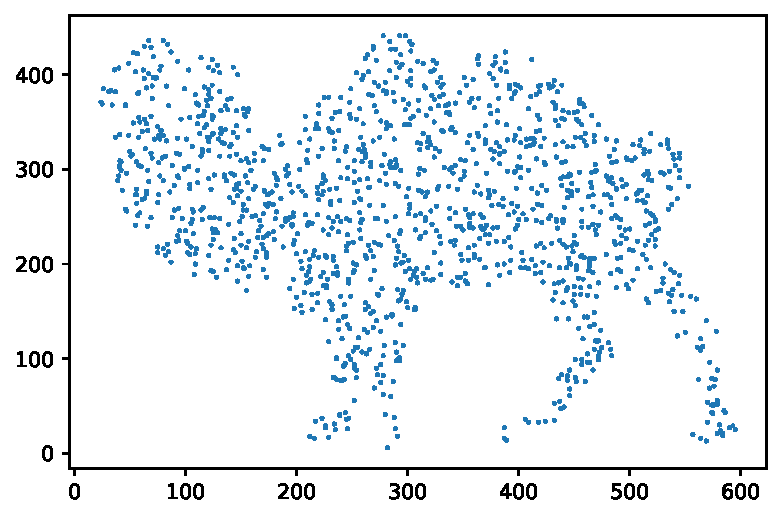
\includegraphics[width=.45\linewidth]{points.pdf}}\hfill
 \subfloat[Delaunay triangulation.]{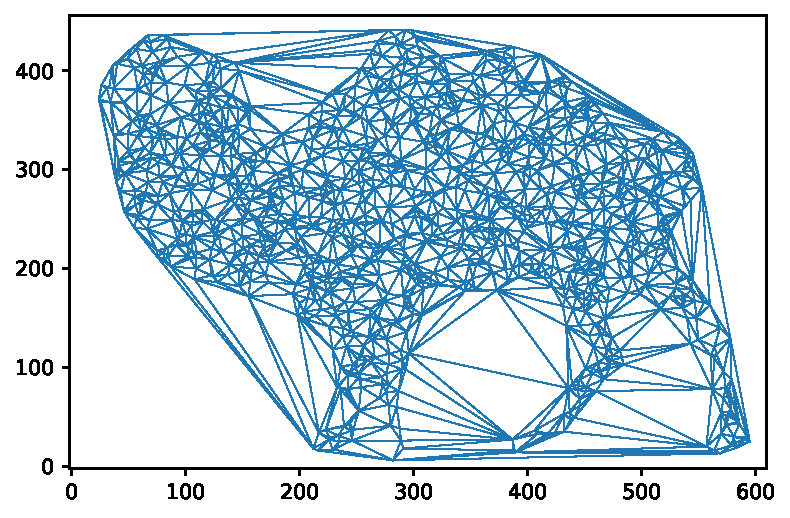
\includegraphics[width=.45\linewidth]{delaunay.pdf}}
 \caption{Set of points and its Delaunay triangulation.}
 \label{fig:alphashape:python:points}
\end{figure}



\subsection{Delaunay triangulation}
The Delaunay triangulation is simply obtained by the following code. The result is presented in Fig.\ref{fig:alphashape:python:points}. 
\begin{python}
tri = Delaunay(points)

# Display result
plt.triplot(points[:,0], points[:,1], tri.simplices, lw=.5)
plt.show()
\end{python}


\subsection{Alpha-solid}
In order to build the alpha-solid, the circum-radii of all triangles should be computed. A rather simple way to do this is to use the class \pinline{Triangle} of \pinline{sympy.geometry}. The use of \pinline{progressbar} displays a progress bar, as the computation might take a long time. The \pinline{sympy} module is a symbolic computation module, and does not an optimal algorithm for this task.

\begin{python}
from sympy.geometry import Triangle
radius=[]
import progressbar
count=0

# takes a long time because of symbolic computation
with progressbar.ProgressBar(max_value=len(tri.simplices)) as bar:
    for t in tri.simplices:
        count+=1
        tt = Triangle(points[t[0], :], points[t[1], :], points[t[2], :] )
        radius.append(tt.circumradius)
        bar.update(count)
\end{python}


Then, given a radius,  one can filter the triangles. The results are presented in Fig.\ref{fig:alphashape:python:ashape}.

\begin{python}
 or R in progressbar.progressbar([5,10, 50, 100, 100000]):
    
    r = np.array(radius)<R
    fig = plt.figure()
    plt.triplot(points[:,0], points[:,1], tri.simplices[r], lw=.5)
    plt.scatter(points[:,0], points[:,1], c='y', s=10)
    plt.show()
\end{python}

\begin{figure}[htbp]
 \centering
 
 \subfloat[$\alpha=1/5$.]{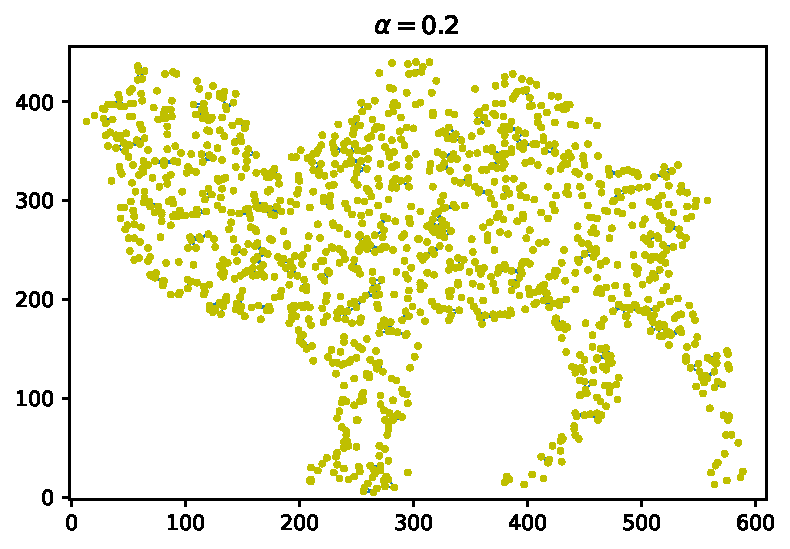
\includegraphics[width=.45\linewidth]{alphashape_5.pdf}}\hfill
 \subfloat[$\alpha=1/10$.]{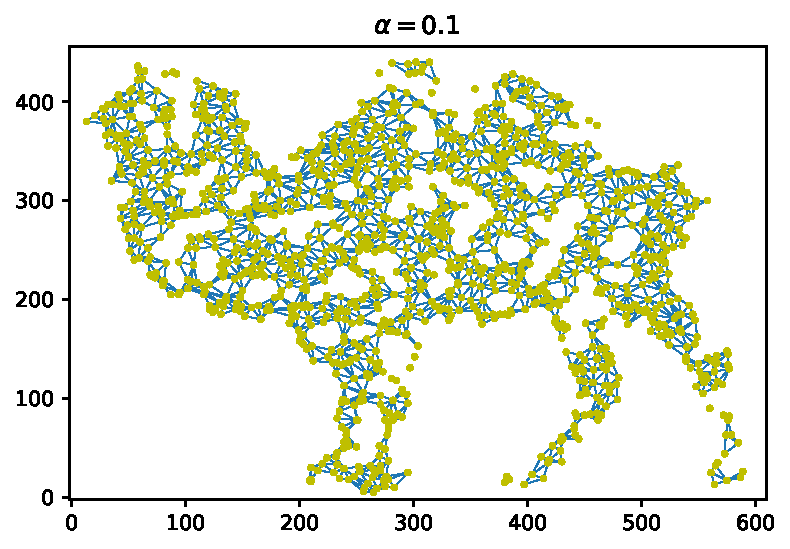
\includegraphics[width=.45\linewidth]{alphashape_10.pdf}}
 
 \subfloat[$\alpha=1/50$.]{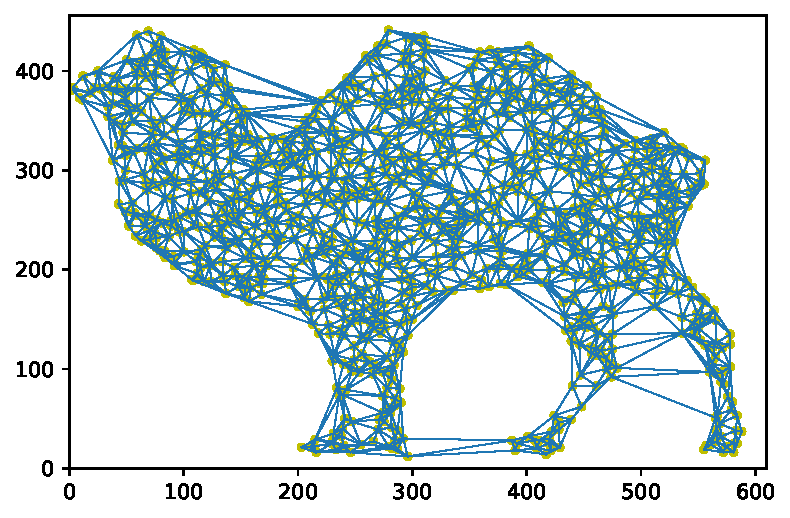
\includegraphics[width=.45\linewidth]{alphashape_50.pdf}}\hfill
 \subfloat[$\alpha=1/100$.]{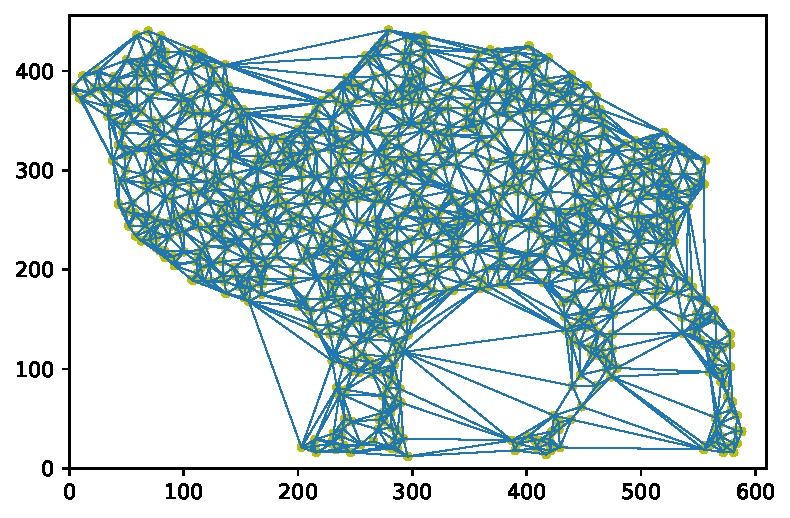
\includegraphics[width=.45\linewidth]{alphashape_100.pdf}}
 
 \subfloat[$\alpha=1/100000$.]{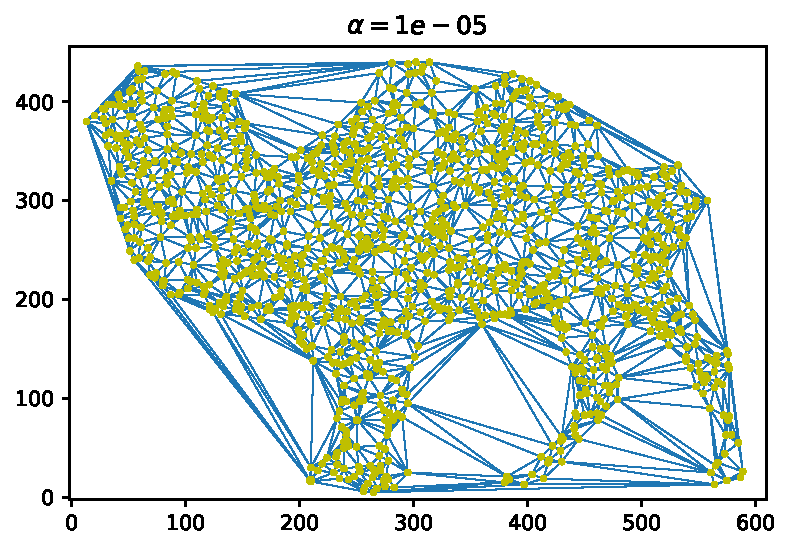
\includegraphics[width=.45\linewidth]{alphashape_100000.pdf}}
 
 \caption{Different alpha-solids.}
 \label{fig:alphashape:python:ashape}
\end{figure}
